\documentclass[aspectratio=169]{beamer}
%\usetheme{CambridgeUS}
%\usecolortheme{beaver}

%\usefonttheme{serif}
%\usepackage{helvet}

\usefonttheme{serif}     % Font theme: serif
%\usepackage{ccfonts}     % Font family: Concrete Math
\usepackage[T1]{fontenc} % Font encoding: T1

\setbeamersize{text margin left=42pt,text margin right=42pt} 
\setbeamertemplate{navigation symbols}{}
\setbeamertemplate{itemize items}[default]

\beamertemplatenavigationsymbolsempty

\definecolor{fore}{RGB}{51,51,51}
\definecolor{back}{RGB}{255, 254, 250}
\definecolor{title}{RGB}{ 255, 15, 0}
\definecolor{links}{RGB}{18, 168, 255}

\setbeamercolor{titlelike}{fg=title}
\setbeamercolor{normal text}{fg=fore,bg=back}
\setbeamercolor{alerted text}{fg=title}
\setbeamercolor{itemize item}{fg=title}
\setbeamercolor{enumerate item}{fg=title}
\hypersetup{colorlinks,urlcolor=links}

% for code https://kbroman.org/blog/2013/10/07/better-looking-latexbeamer-slides/
\usepackage{listings}
\definecolor{keywords}{RGB}{255,0,90}
\definecolor{comments}{RGB}{60,179,113}
\lstset{language=Python,
keywordstyle=color{keywords},
commentstyle=color{comments}emph}

% fonts
\usepackage[sc]{mathpazo}


% title info
\title{\textbf{1. Maps For Navigation / 2. Sustainability}}
\subtitle{\textbf{GGR424 - Transportation Geography \& Planning}}
\author{Jeff Allen}
\institute{University of Toronto}
\date{February 28, 2022}




\begin{document}
	
\begin{frame}
	\titlepage	
\end{frame}





\begin{frame}
	
	\textbf{Announcements}
	
	\begin{itemize}
		\item Transportation data analysis assignment due March 3
		\item Project Proposal due March 10
		\item Monday office hours 3:30pm to 5:00pm in SS5060 (I'll also keep my Zoom room open during this time)
		\item Friday office hours still only on Zoom, 2:30pm to 3:30pm
	\end{itemize}
	
\end{frame}





\begin{frame}
	
	\textbf{Today}
	
	\begin{itemize}
		\item Maps for navigation
		\item Chat about final project
		\item Sustainable transport
	\end{itemize}
	
\end{frame}




\begin{frame}
	
	
	\begin{columns}
		
		\begin{column}{0.32\textwidth}
			
			\textbf{Maps for navigation}
			
			\vspace{8mm}
			
			"Stick Charts" from the Marshall Islands
			
			\begin{itemize}
				\item Shells represent islands
				\item Sticks represent ocean swells and wave-crests
			\end{itemize}
			
		\end{column}
		
		\begin{column}{0.68\textwidth}
			\begin{figure}
				\centering
				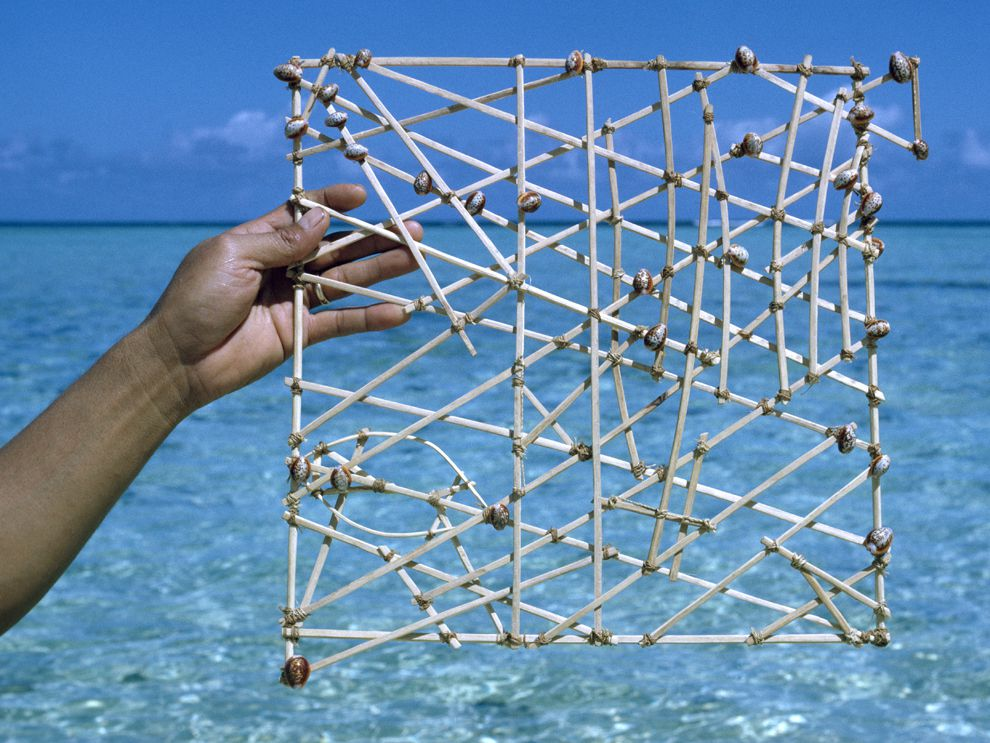
\includegraphics[width=0.99\linewidth]{images/marshall_stick_chart.jpg}
			\end{figure}
			
		\end{column}
		
	\end{columns}
	
	\vspace{2mm}
	\tiny More info: \url{http://marshall.csu.edu.au/MJHSS/Issue2005/MJHSS2005_103.pdf}
	
\end{frame}






\begin{frame}
	
	
	
	\begin{columns}
		\begin{column}{0.6\textwidth}
			
			\textbf{Maps for navigation}
			
			\vspace{8mm}
			
			Peutinger Table
			\vspace{3mm}
			\begin{itemize}
				\item a road map of the Roman Empire 
				\item (this is a 13th century copy of an unknown original) 
			\end{itemize} 
		\end{column}
		
		\begin{column}{0.4\textwidth}
			\begin{figure}
				\centering
				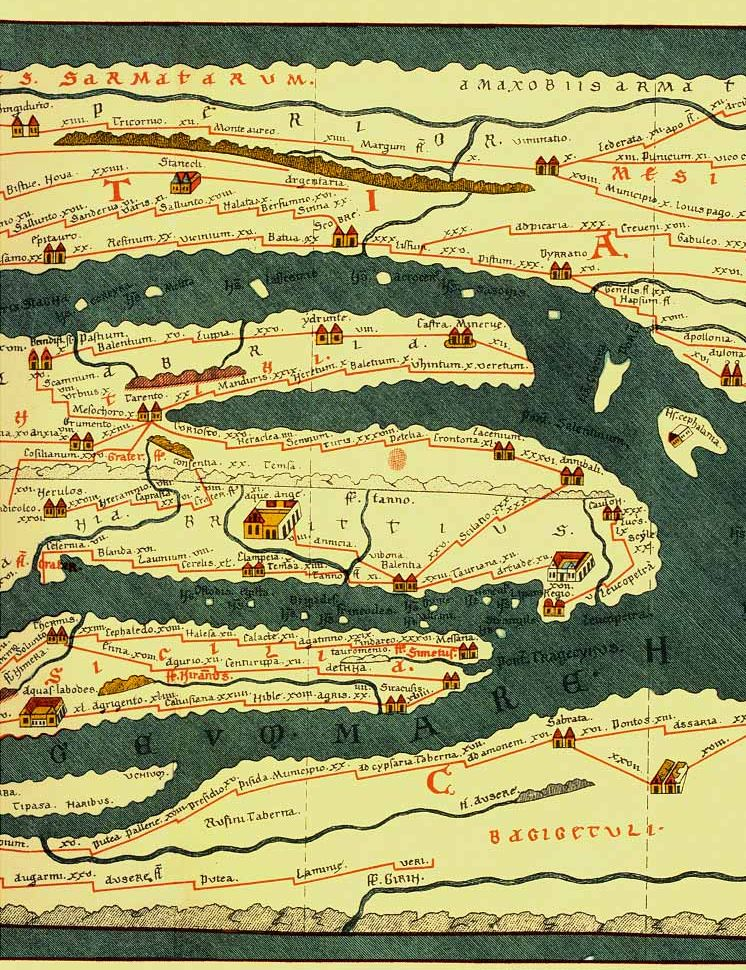
\includegraphics[width=1\linewidth]{images/Part_of_Tabula_Peutingeriana.jpg}
			\end{figure}
			\tiny Source: \url{https://commons.wikimedia.org/wiki/File:TabulaPeutingeriana.jpg}
		\end{column}
		
		
	\end{columns}
	
\end{frame}



\begin{frame}
	\textbf{Maps for navigation} - e.g. 20th and early 21st century road maps 
	
	\begin{figure}
		\centering
		\includegraphics[width=1\linewidth]{images/map_book_scarborough_edit.jpg}
	\end{figure}
	
	\tiny Map Art (2010) Toronto \& Area street guide
	
\end{frame}


\begin{frame}
	\textbf{Maps for navigation} - e.g. TTC System Map
	
	\begin{figure}
		\centering
		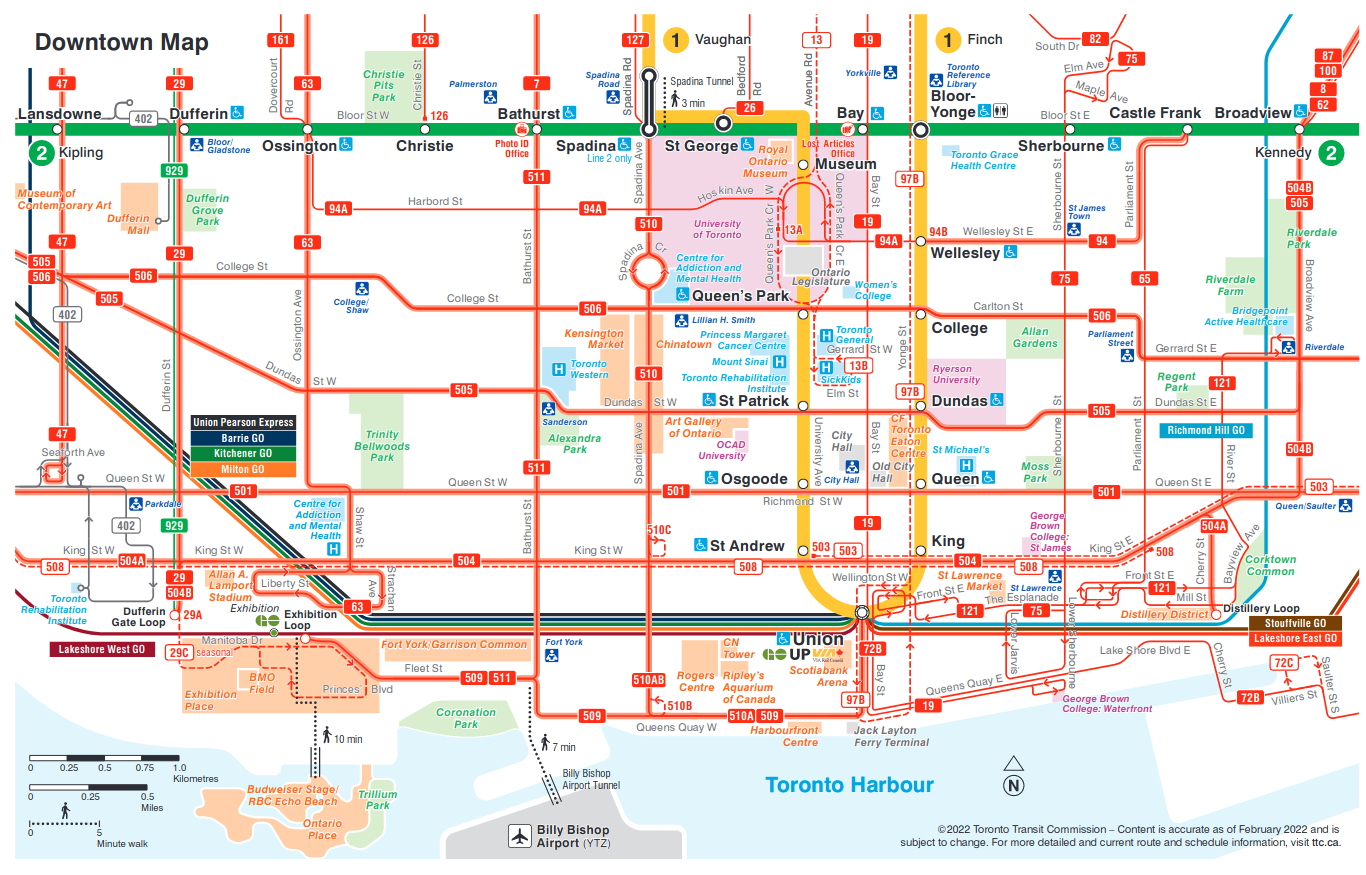
\includegraphics[width=0.86\linewidth]{images/ttc_downtown.png}
	\end{figure}
	
	\tiny \url{https://www.ttc.ca/routes-and-schedules}
\end{frame}




\begin{frame}
	\textbf{Maps for navigation} - e.g. Google Maps
	
	\begin{figure}
		\centering
		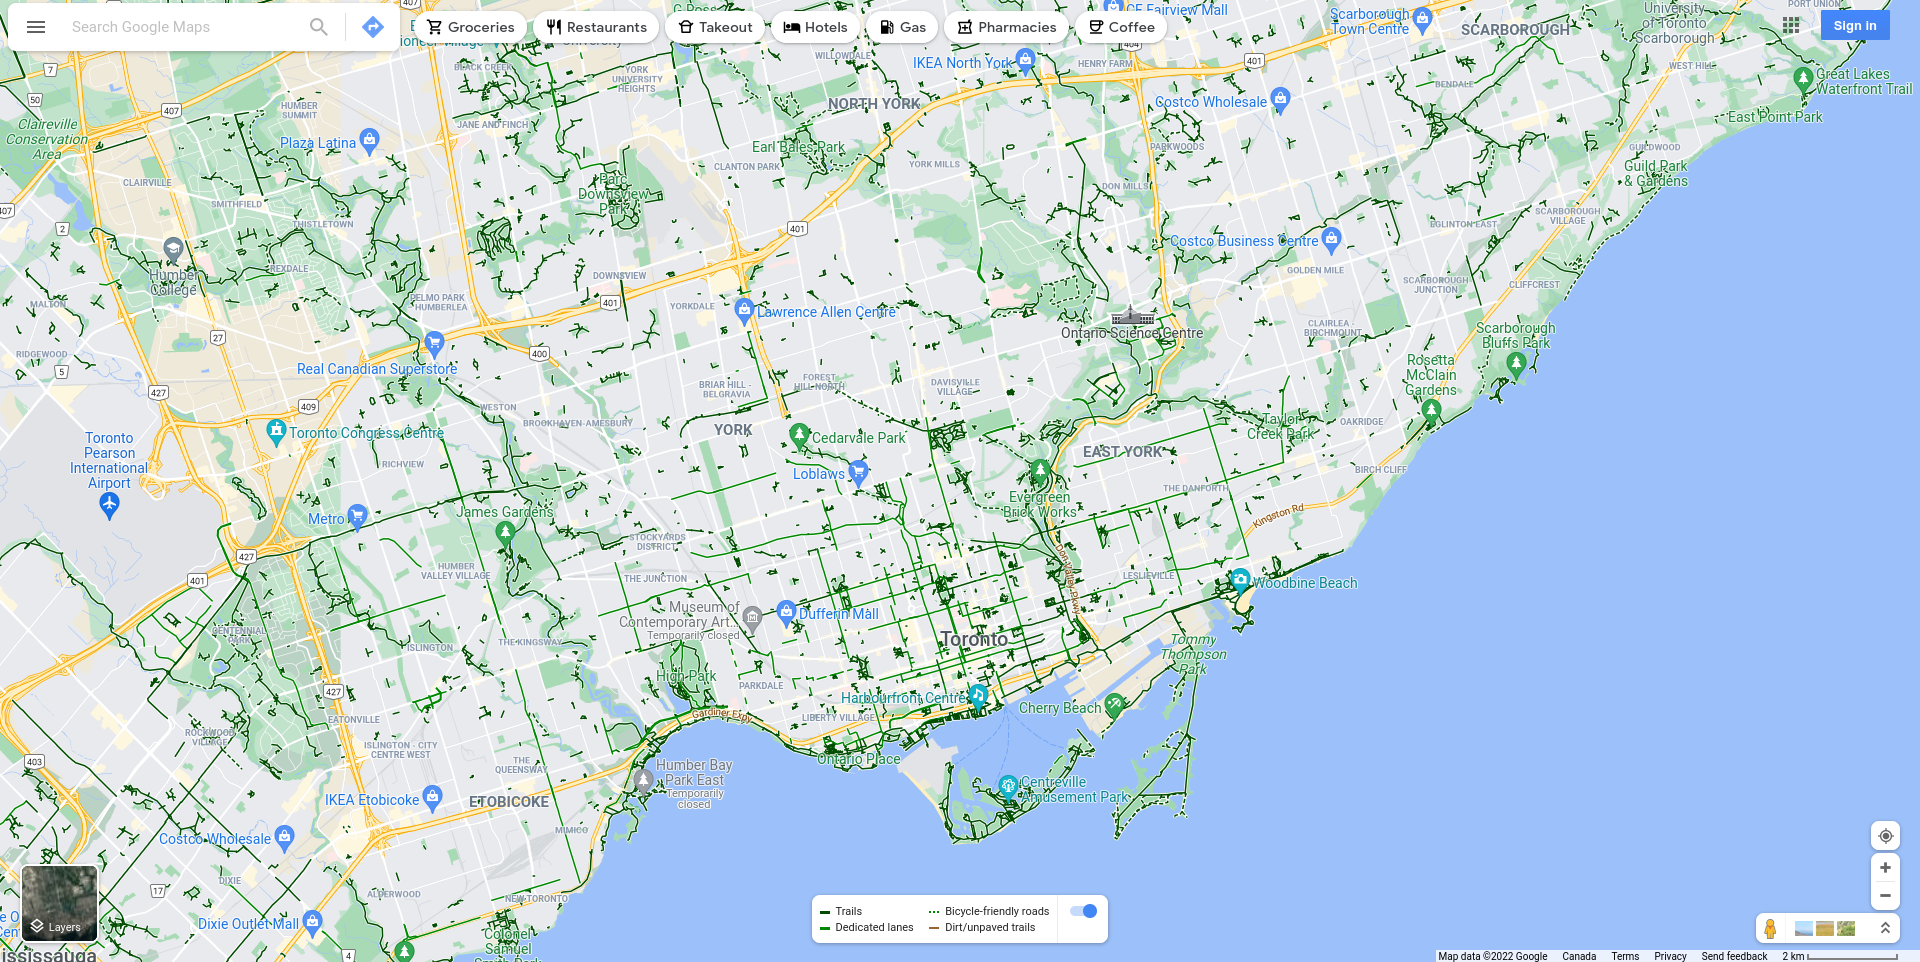
\includegraphics[width=1\linewidth]{images/google_maps_toronto.png}
	\end{figure}
	
	\tiny \url{https://www.google.ca/maps/@43.6574817,-79.4021975,13.25z}
\end{frame}





\begin{frame}
	
	What are the design elements that make a good navigational map?
	
\end{frame}


%\begin{frame}
%	
%	Network hierarchy (of edges and nodes)
%	
%	Distinguishing routes
%	
%	Network connectivity
%
%   Highlight key detsinantions 
%
%   Geograpahic reference, maybe
%	
%\end{frame}


\begin{frame}
	
		\begin{figure}
			\centering
			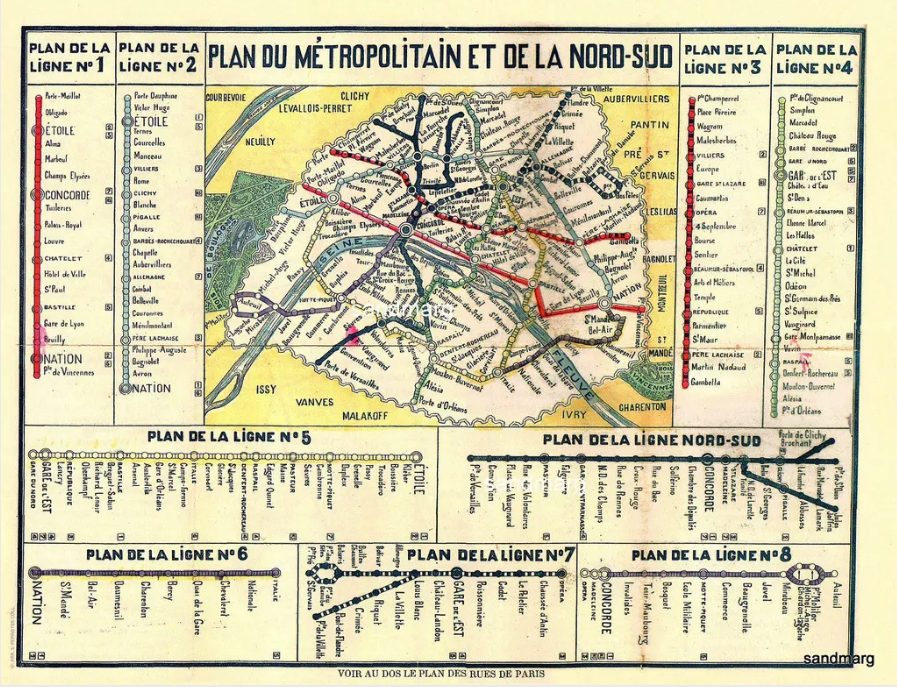
\includegraphics[width=0.8\linewidth]{images/paris_1913.png}
		\end{figure}
	
		\tiny Shared by Megan Belisle
		
		\tiny \url{https://transitmap.net/paris-metro-1913/}
	
\end{frame}






\begin{frame}
	
	\begin{figure}
		\centering
		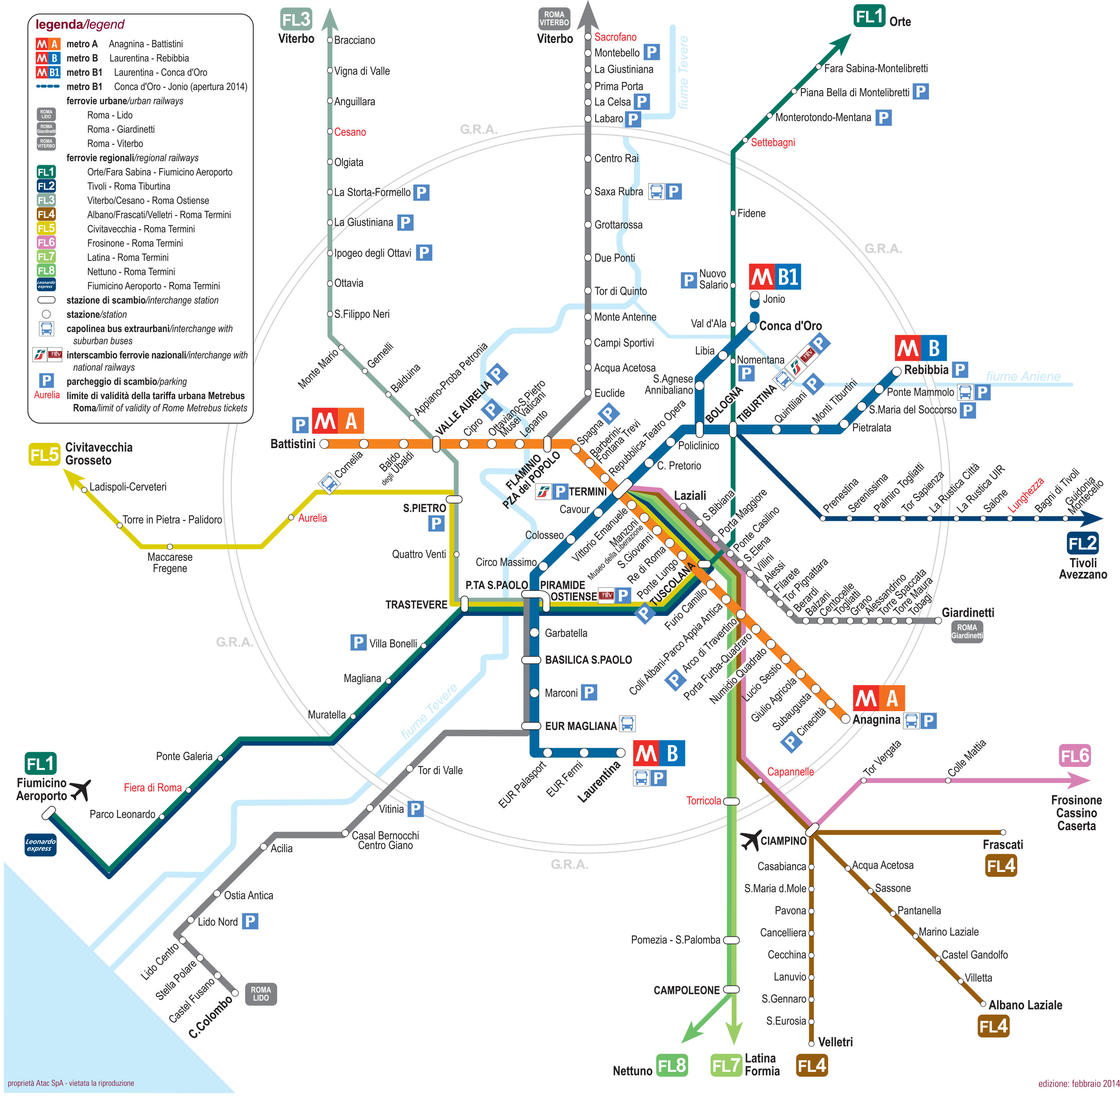
\includegraphics[width=0.6\linewidth]{images/rome-train-map.jpeg}
	\end{figure}
	
	\tiny Shared by Steven Kakaletris
	
	\tiny \url{https://romemap360.com/rome-train-map}
	
\end{frame}




\begin{frame}
	
	\begin{figure}
		\centering
		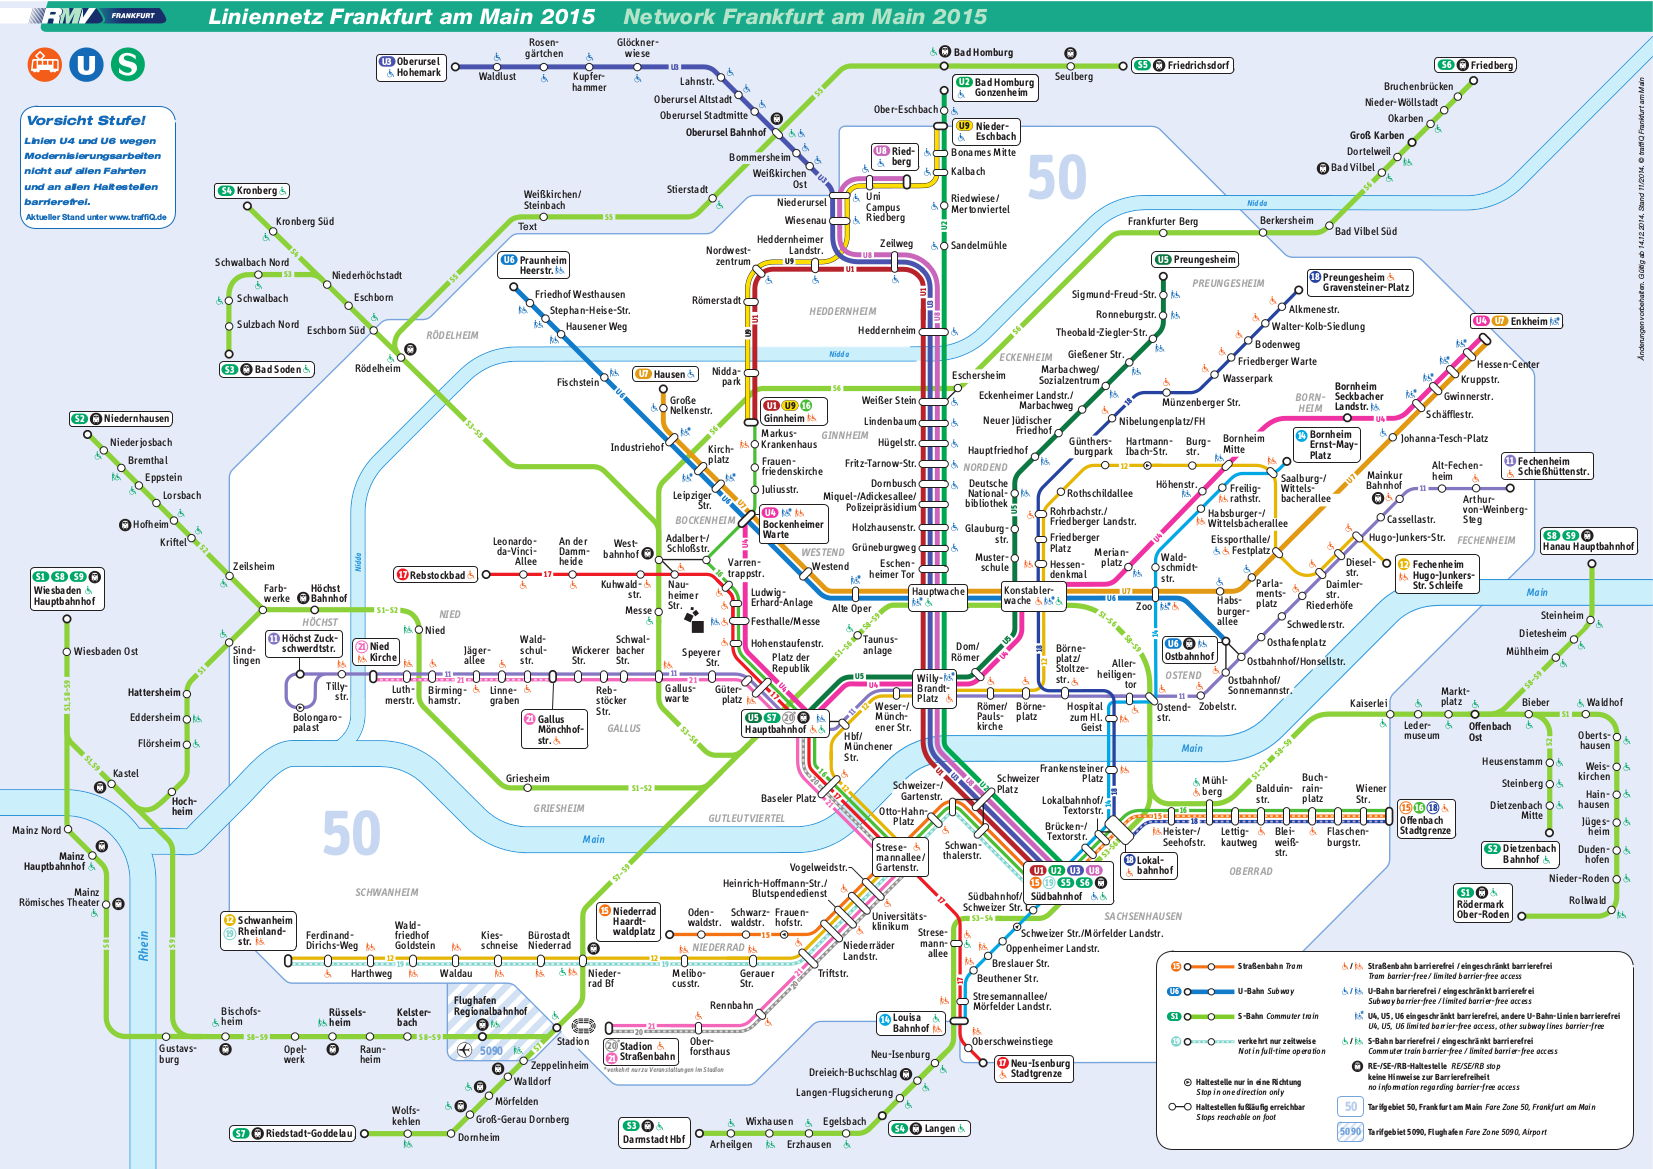
\includegraphics[width=0.86\linewidth]{images/frankfurt.jpg}
	\end{figure}
	
	\tiny Shared by Code Hale
	
	\tiny \url{https://mapa-metro.com/en/germany/frankfurt/frankfurt-u-bahn-map.htm}
	
\end{frame}



\begin{frame}
	
	\begin{figure}
		\centering
		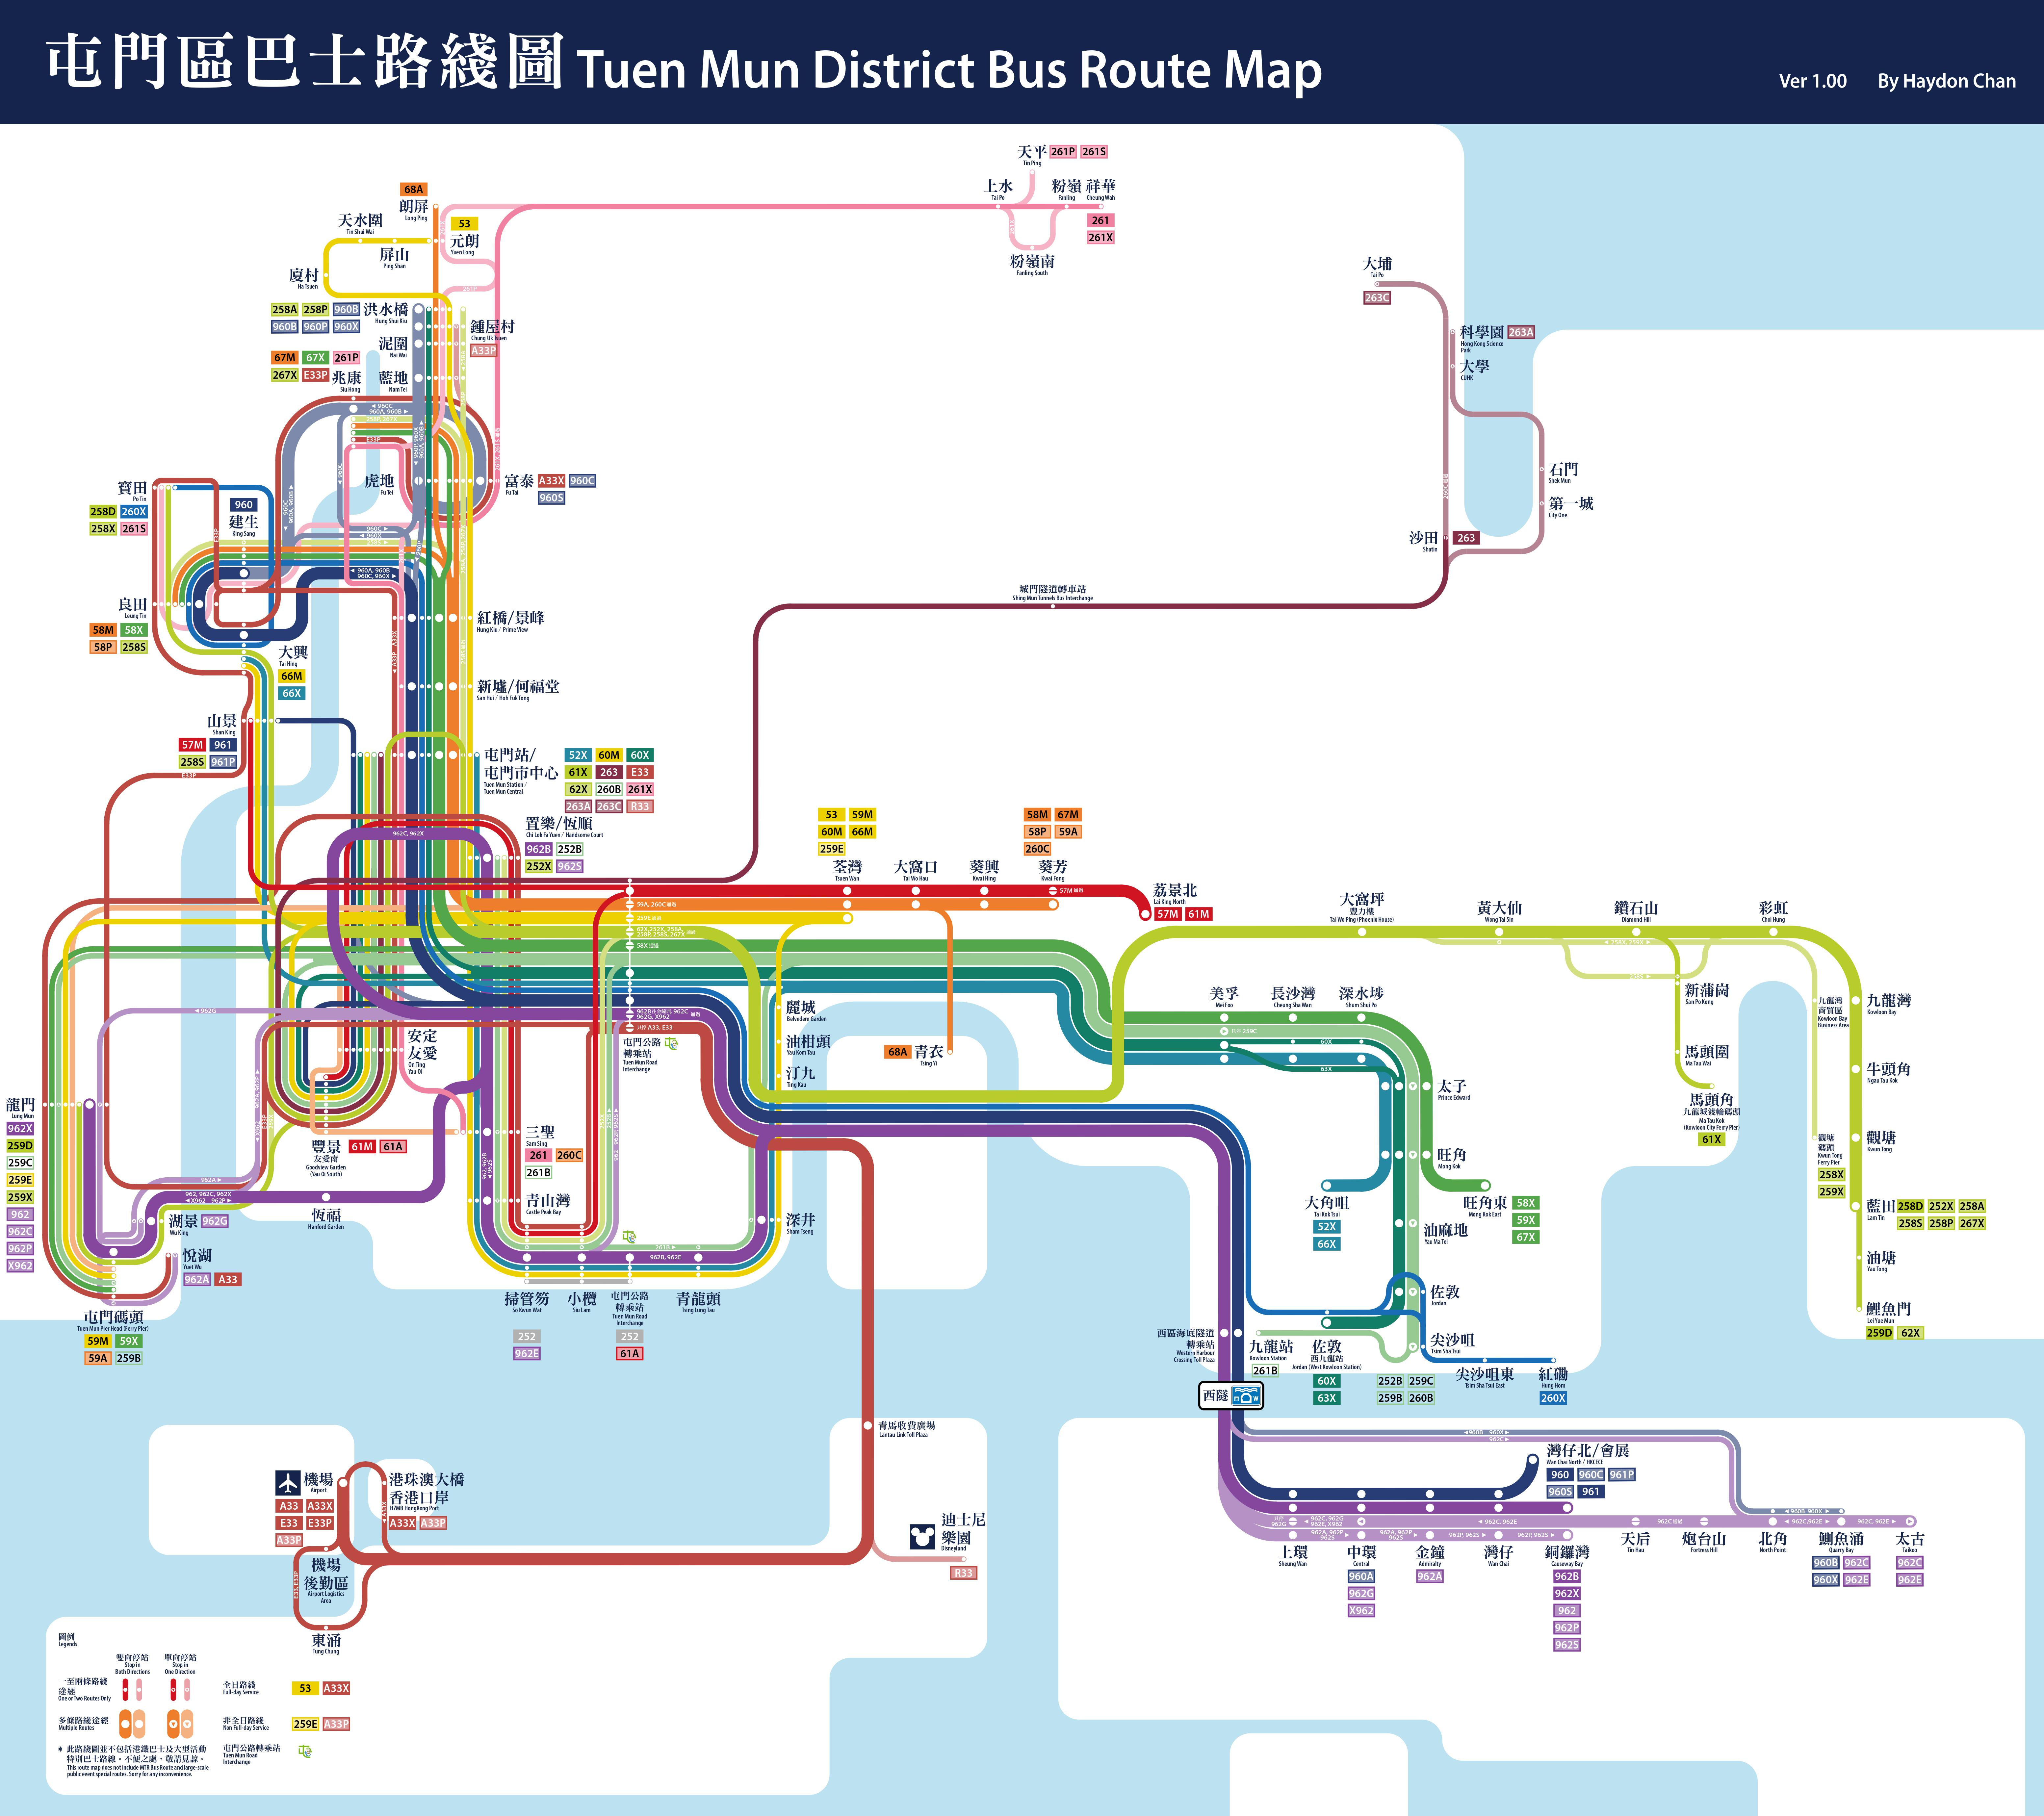
\includegraphics[width=0.68\linewidth]{images/hong_kong_bus.jpg}
	\end{figure}
	
	\tiny Shared by Tung Ki Yeung
	
	\tiny \url{https://www.behance.net/gallery/96041633/Tuen-Mun-District-Bus-Route-Map-Design}
	
\end{frame}










\begin{frame}
	
	Navigational maps have to balance between detail and legibility
	
	\vspace{6mm}
	
	\textbf{Cartographic Selection}
	
	\begin{itemize}
		\item deciding what layers to include on a map, and what not to include
	\end{itemize}
	
	 \textbf{Cartographic Generalization}
	\begin{itemize}
		\item simplifying the precision and detail of features to only show what's essential
		\item e.g. smoothing a line
		\item e.g. merging areas, aggregating points
		\item e.g. reclassifying data
		\item e.g. exaggerating features
	\end{itemize}
	
\end{frame}




\begin{frame}
	
	\begin{figure}
		\centering
		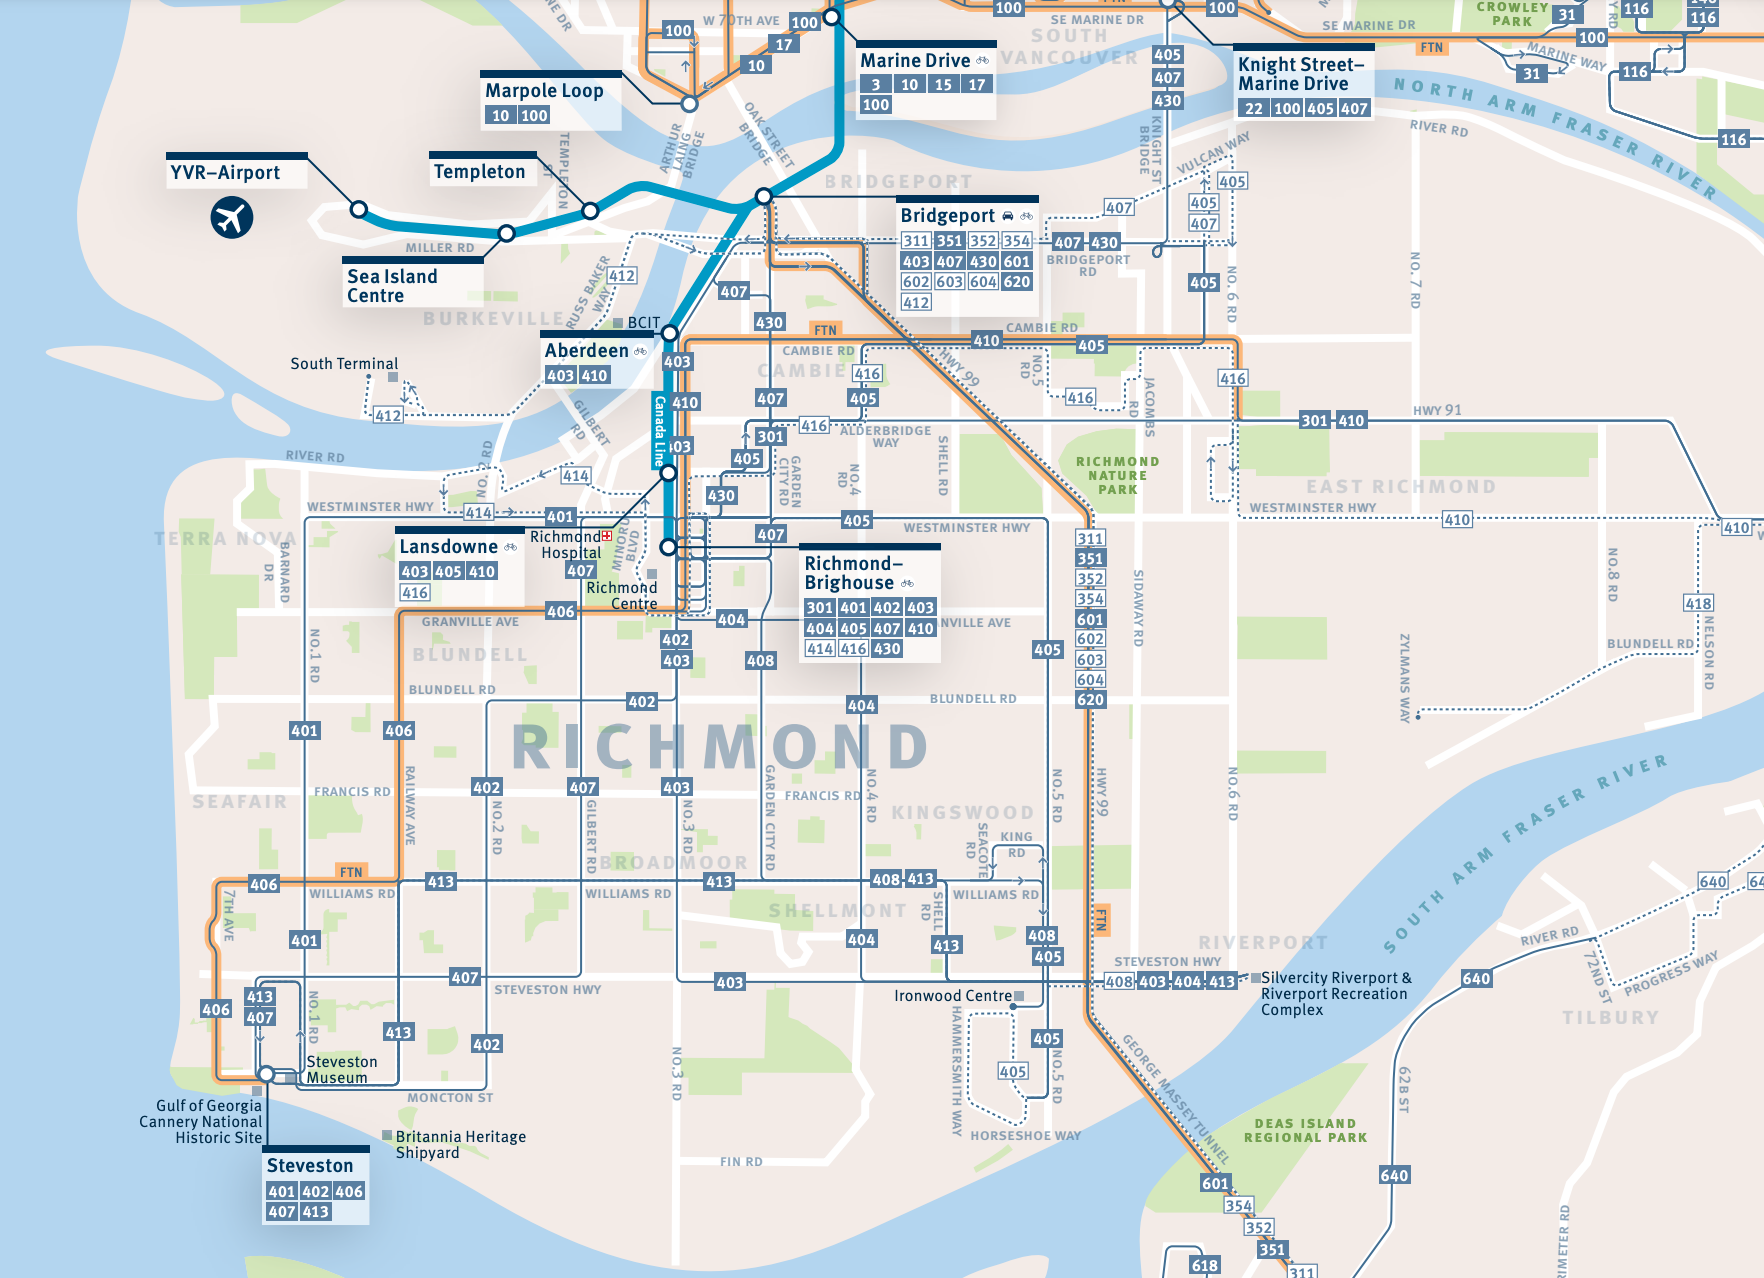
\includegraphics[width=0.8\linewidth]{images/richmond.png}
	\end{figure}
	
	\tiny Shared by Angel Yang 
	
	\tiny \url{https://www.translink.ca/-/media/translink/documents/schedules-and-maps/transit-system-maps/regional-maps/january-2022/rdt_2022-01-03.pdf}
	
\end{frame}


\begin{frame}
	
	\begin{figure}
		\centering
		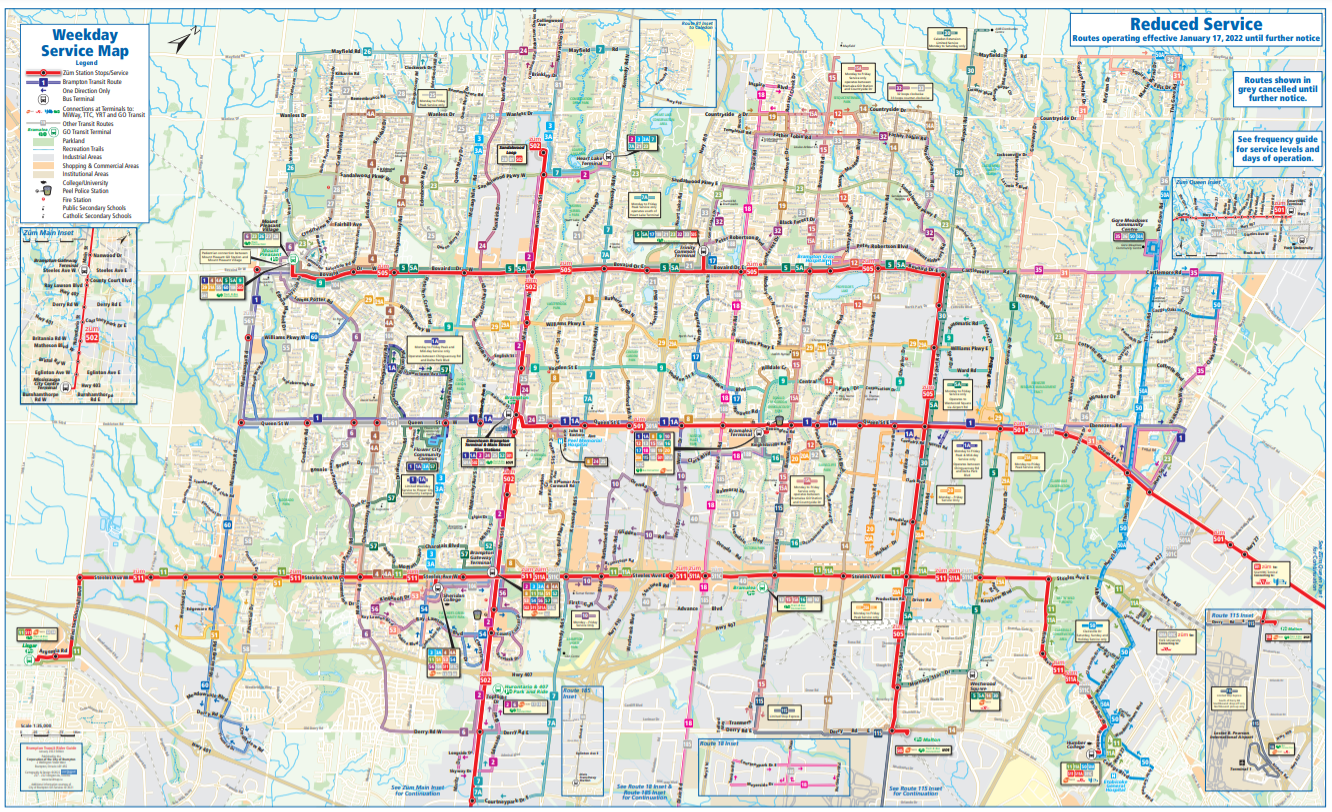
\includegraphics[width=0.93\linewidth]{images/brampton_map.png}
	\end{figure}
	
	\tiny Shared by Erika Lindsay 
	
	\tiny \url{https://www.brampton.ca/EN/residents/transit/plan-your-trip/Documents/Brampton_System_M-F_Jan2022.pdf}
	
\end{frame}








\begin{frame}
	
	e.g. Bike Map in Cincinnati
	
	\begin{figure}
		\centering
		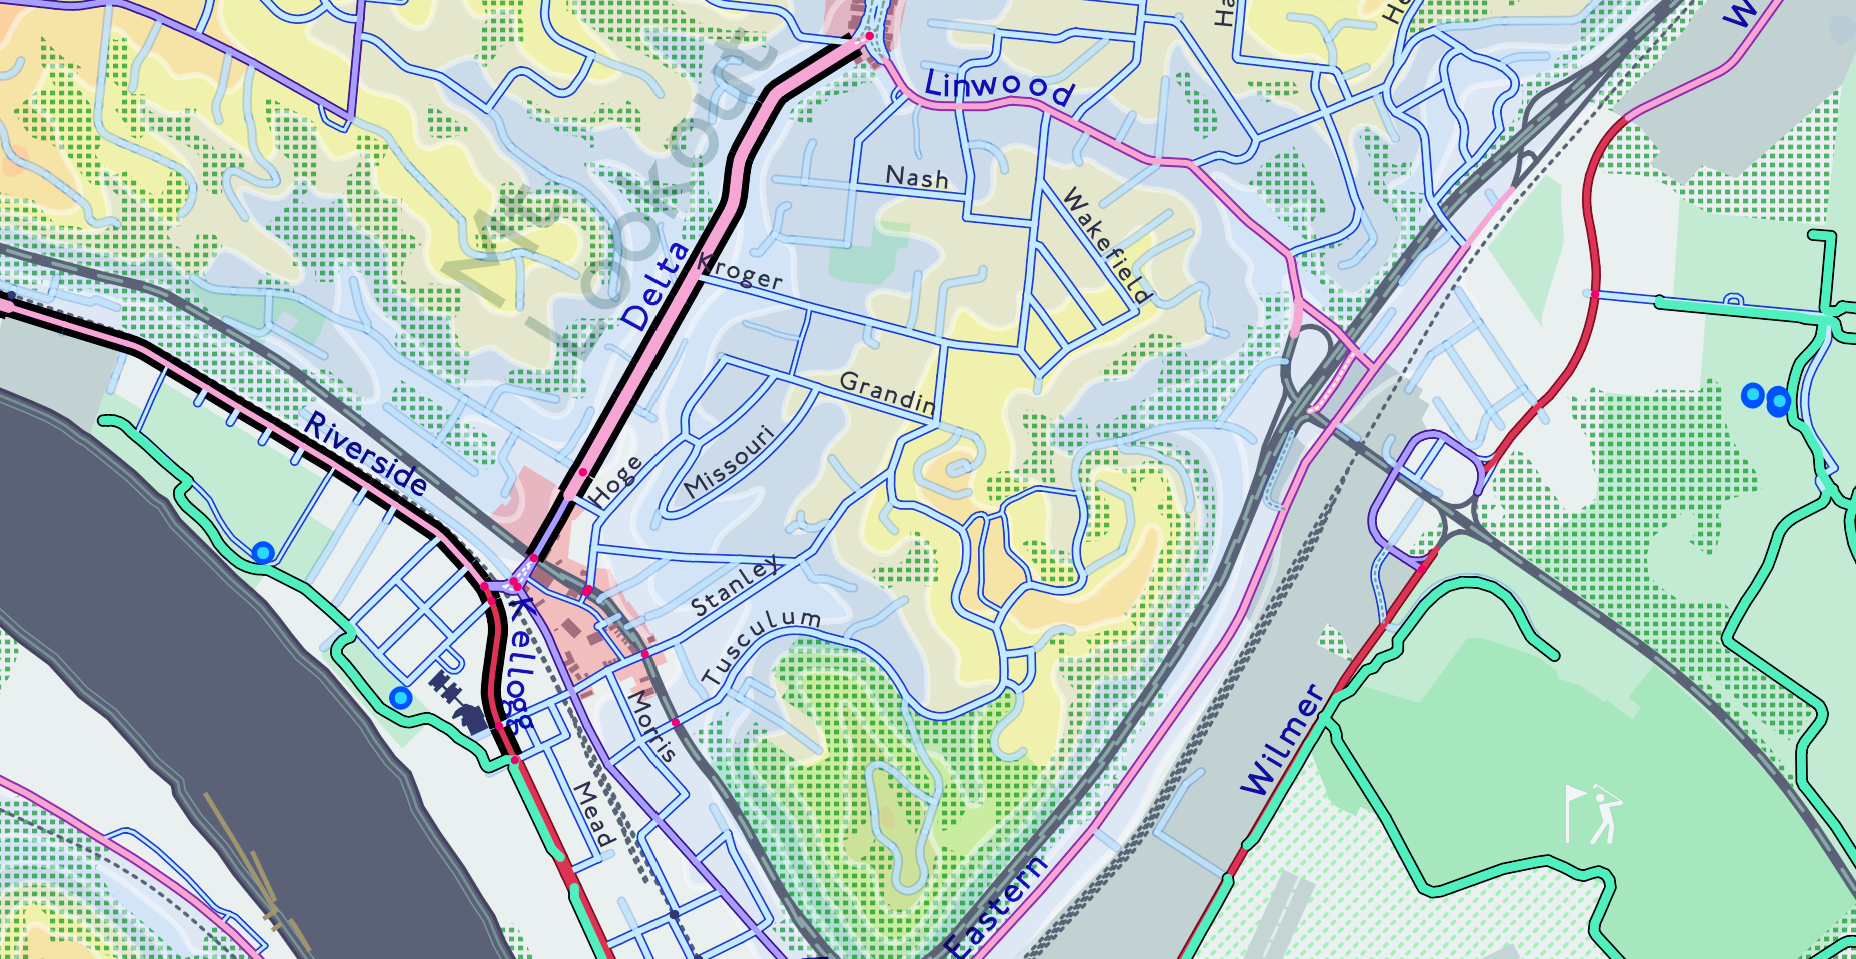
\includegraphics[width=1\linewidth]{images/bike_map_1.png}
	\end{figure}
	
	\tiny \url{https://www.cincymap.org/cbm/}
	
\end{frame}





\begin{frame}
	
	e.g. Bike Map in Cincinnati
	
	\begin{figure}
		\centering
		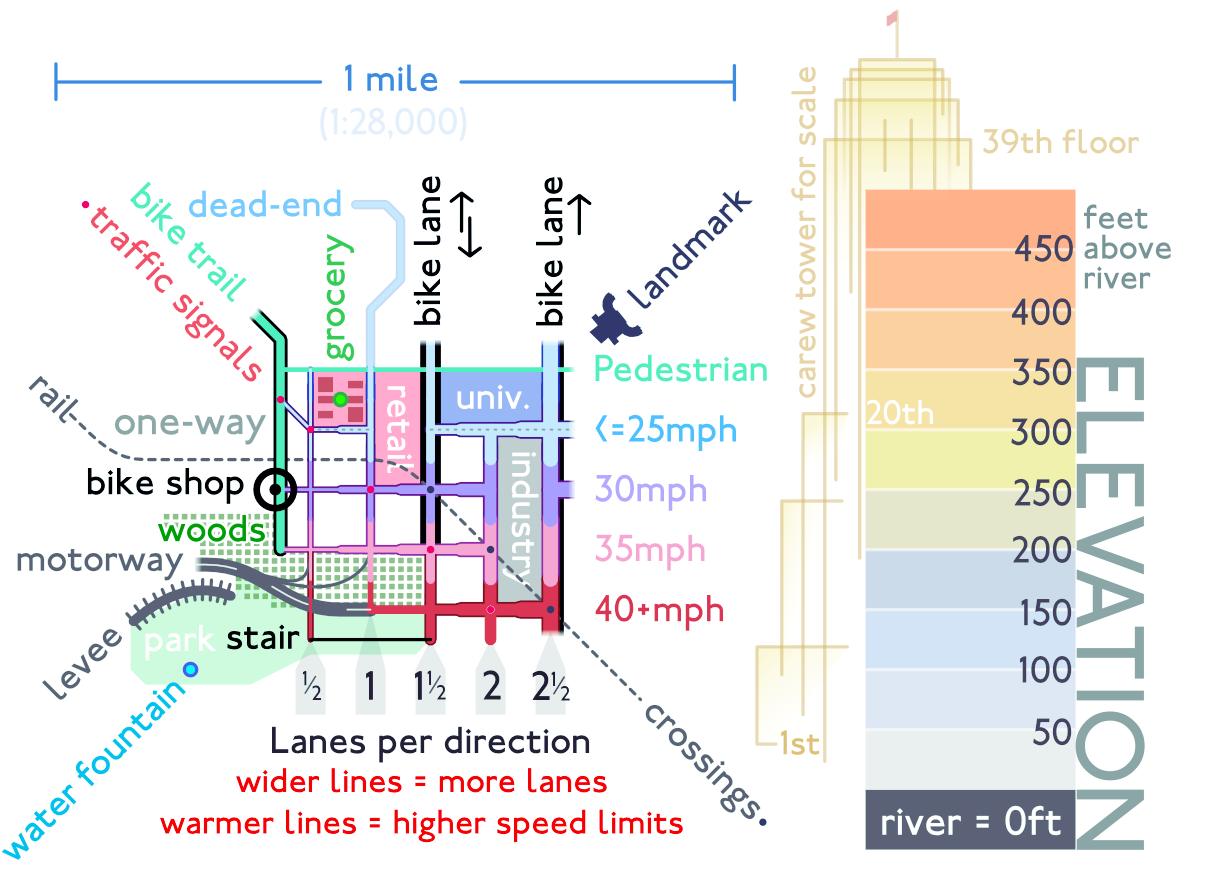
\includegraphics[width=0.8\linewidth]{images/bike_map_leg.png}
	\end{figure}
	
	\tiny \url{https://www.cincymap.org/cbm/}
	
\end{frame}




\begin{frame}
	
	Its challenging to add data density, but without compromising legibility
	
	\vspace{2mm}
		e.g. Frequency on transit maps
	\begin{figure}
		\centering
		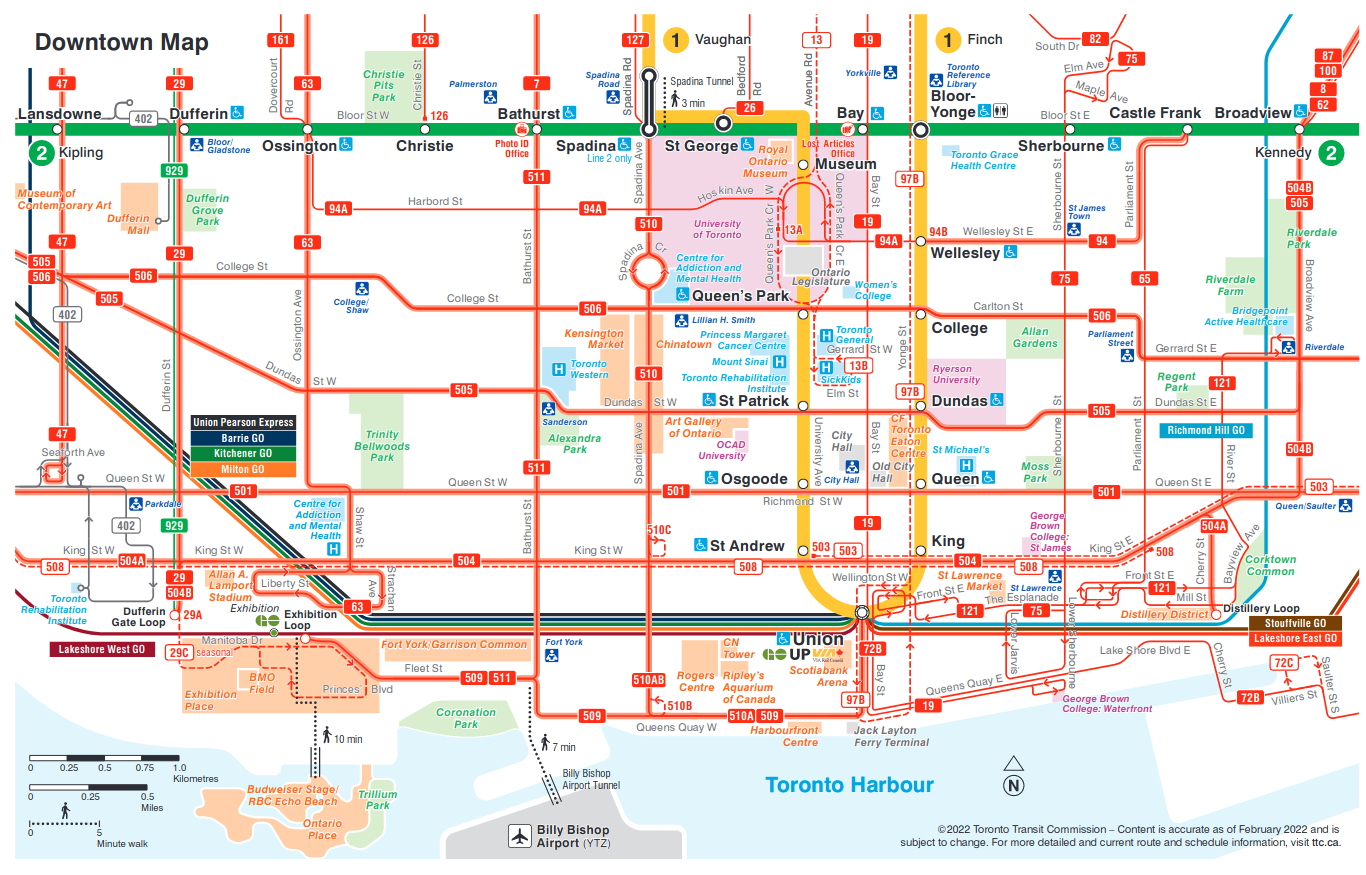
\includegraphics[width=0.84\linewidth]{images/ttc_downtown.png}
	\end{figure}
	
	\tiny \url{https://www.ttc.ca/routes-and-schedules}
	
\end{frame}




\begin{frame}
	
	\begin{figure}
		\centering
		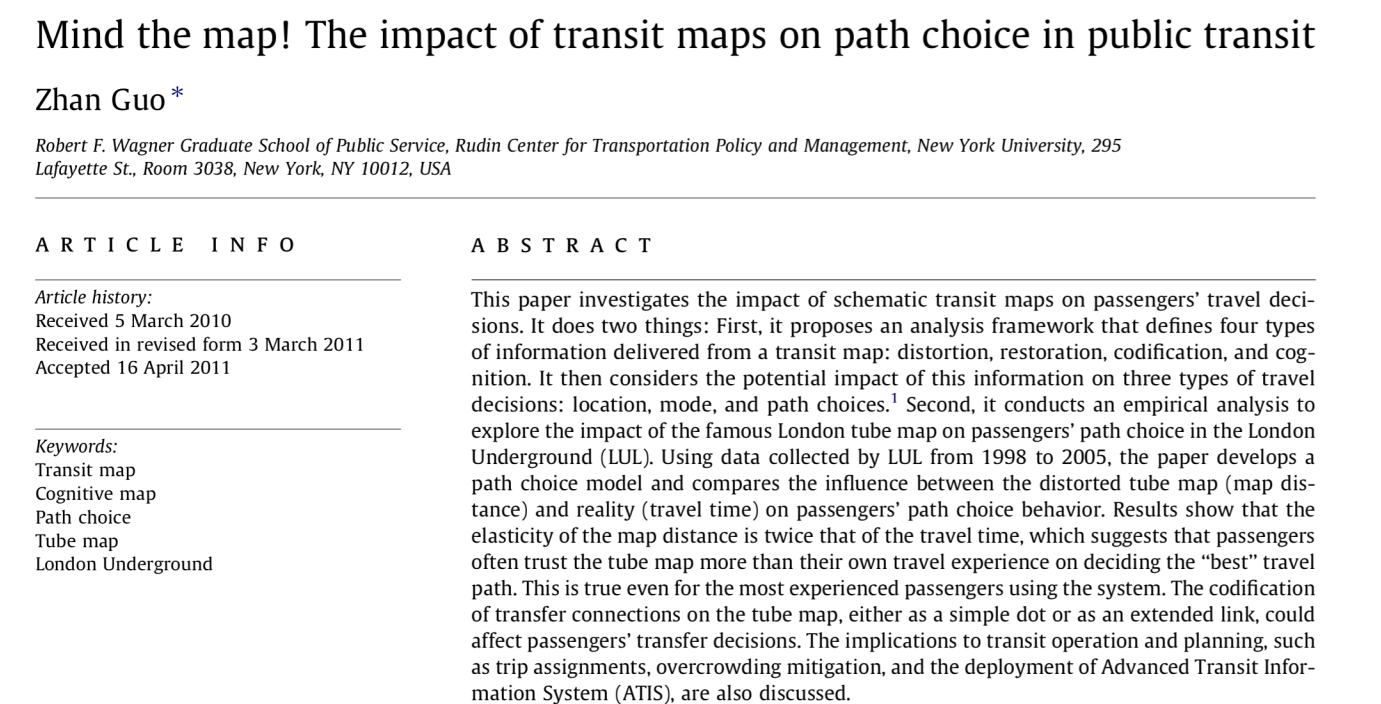
\includegraphics[width=0.88\linewidth]{images/mind-the-map.png}
	\end{figure}
	
\end{frame}







\begin{frame}
	
	\textbf{Transportation improvement plan}
	
	\vspace{2mm}
	
	For the final project in this class, you will propose an intervention, solution, or improvement to a transportation problem
	
	\vspace{2mm}
	
	\begin{itemize}
		\item (5\%) Project Proposal due March 10
		\item (5\%) Presentations March 28 and April 4
		\item (25\%) Final Report due April 8
	\end{itemize}
	
\end{frame}





\begin{frame}
	
	\textbf{Transport and the Environment:}

		\begin{figure}
			\centering
			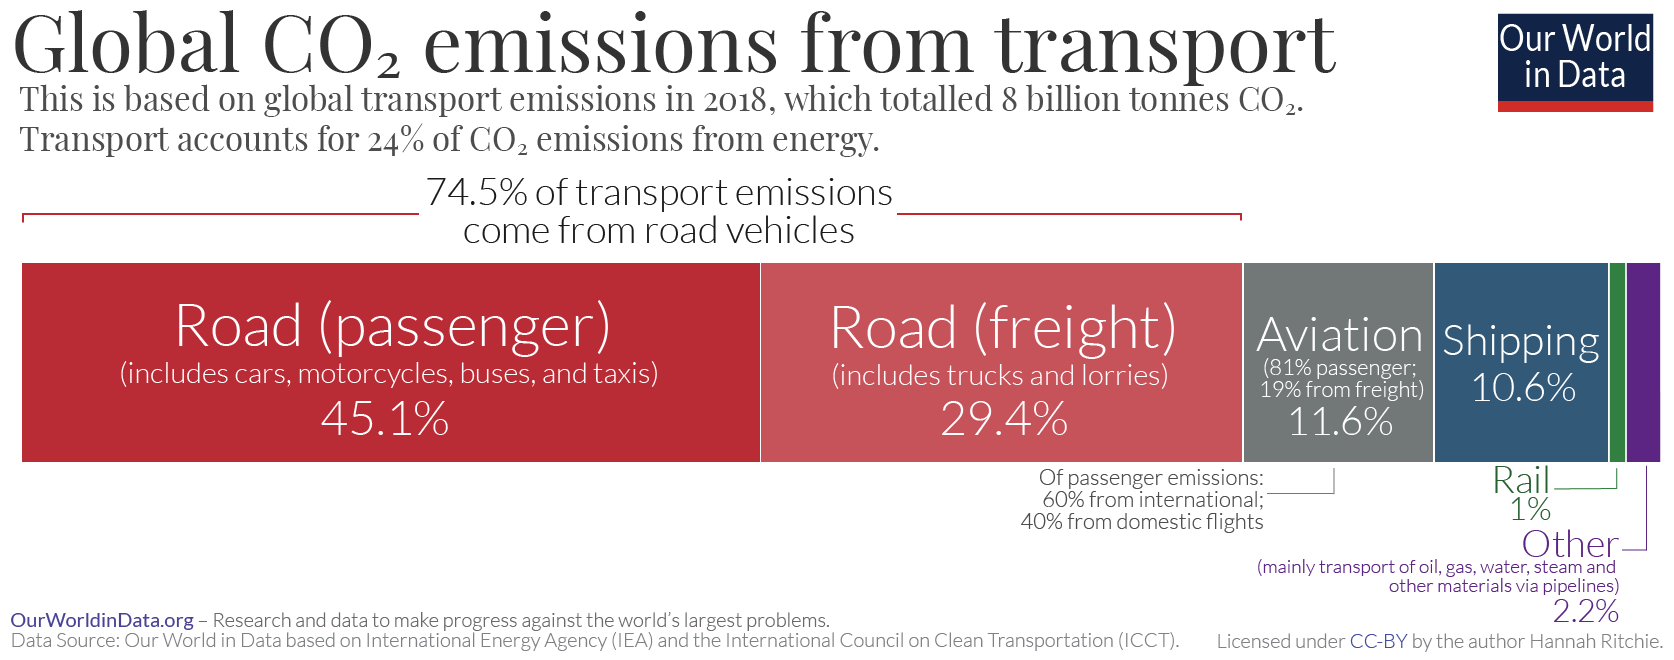
\includegraphics[width=0.98\linewidth]{images/Transport-CO2-emissions-by-mode-bar-chart.png}
		\end{figure}
	
\end{frame}



\begin{frame}
	
	\textbf{Transport and the Environment:}
	
	\begin{figure}
		\centering
		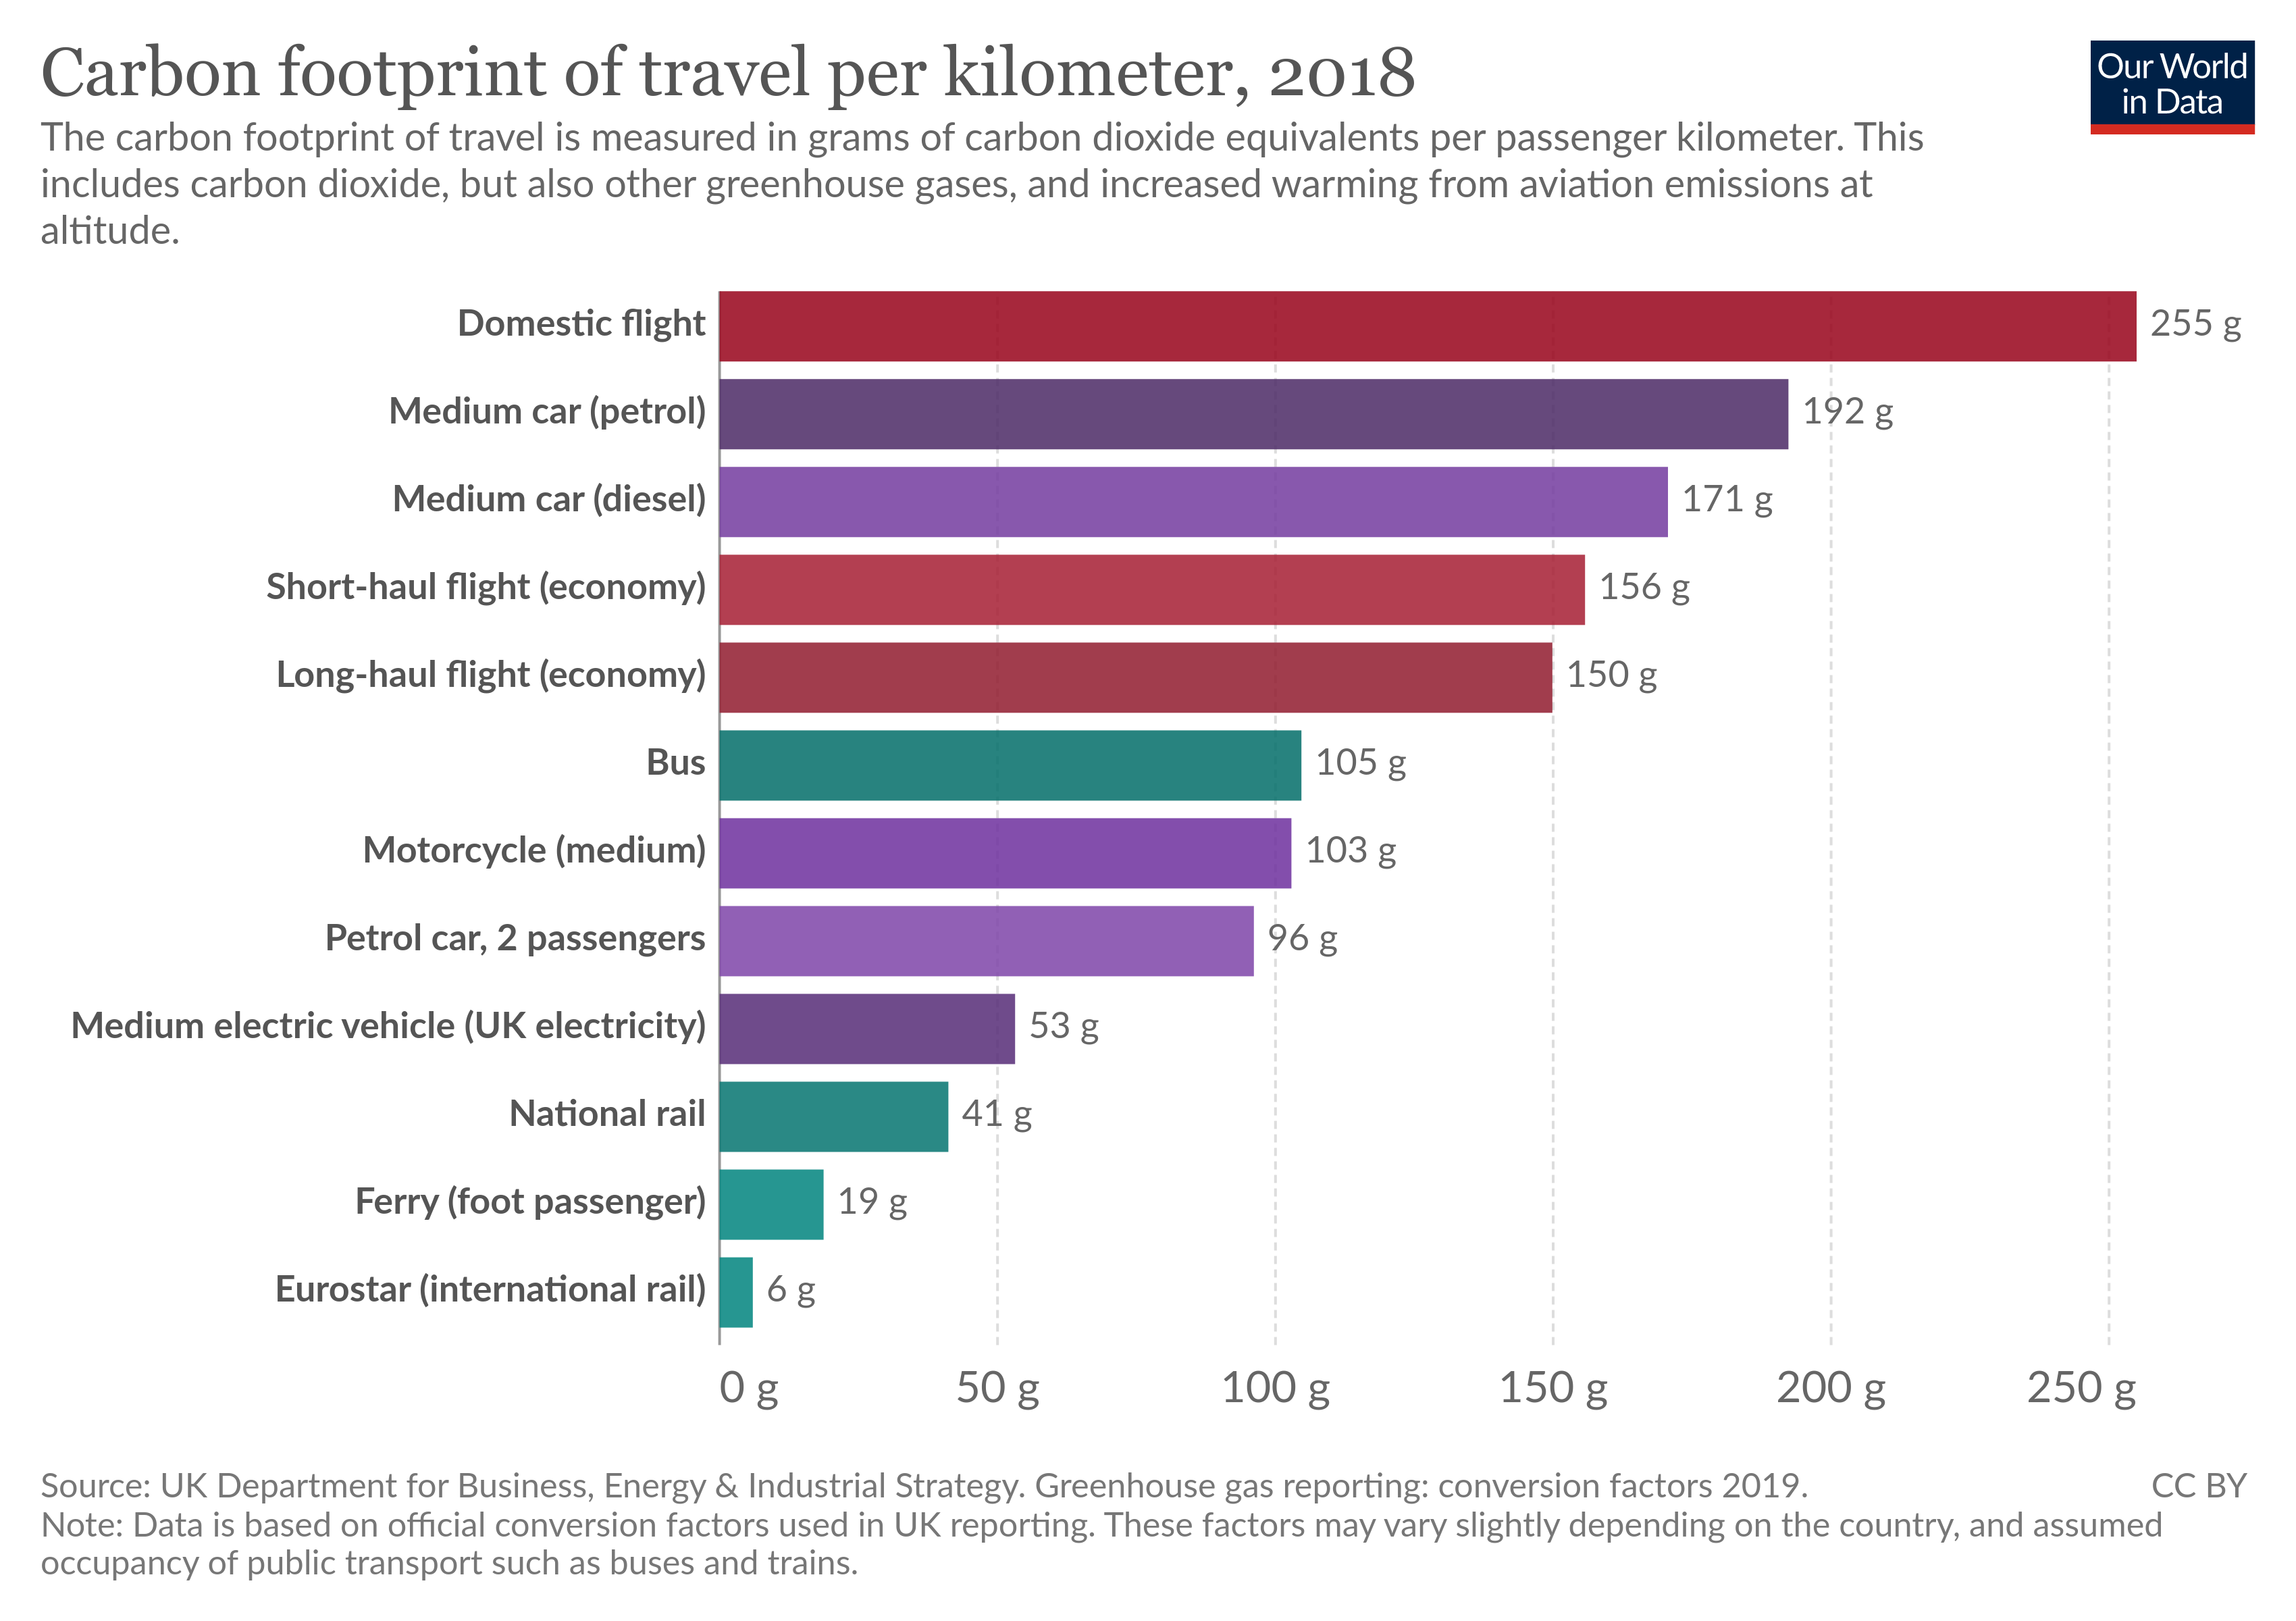
\includegraphics[width=0.84\linewidth]{images/carbon-footprint-travel-mode.png}
	\end{figure}

	\tiny\url{https://ourworldindata.org/travel-carbon-footprint}
	
\end{frame}




\begin{frame}
	
	\textbf{How can we make urban transport more sustainable?}
	
	\vspace{6mm}
	
	\textbf{Avoid}
	\begin{itemize}
		\item Avoiding (long distance) trips (by car)
		\item Banister (2011) Section 5.1 and 5.3
		\item i.e. system efficiency
	\end{itemize}

	\textbf{Shift}
	\begin{itemize}
		\item Shifting trips to more sustainable modes
		\item Banister (2011) Section 5.2
		\item i.e. trip efficiency
	\end{itemize}

	\textbf{Improve}
	\begin{itemize}
		\item Improving the efficiency (i.e. reducing the impacts) of existing transport options
		\item Banister (2011) Section 5.4
		\item i.e. vehicle efficiency
	\end{itemize}

	\vspace{2mm}
	
	\tiny{Banister (2008) Cities, mobility and climate change}
	
	
\end{frame}



\begin{frame}
	
	\begin{figure}
		
		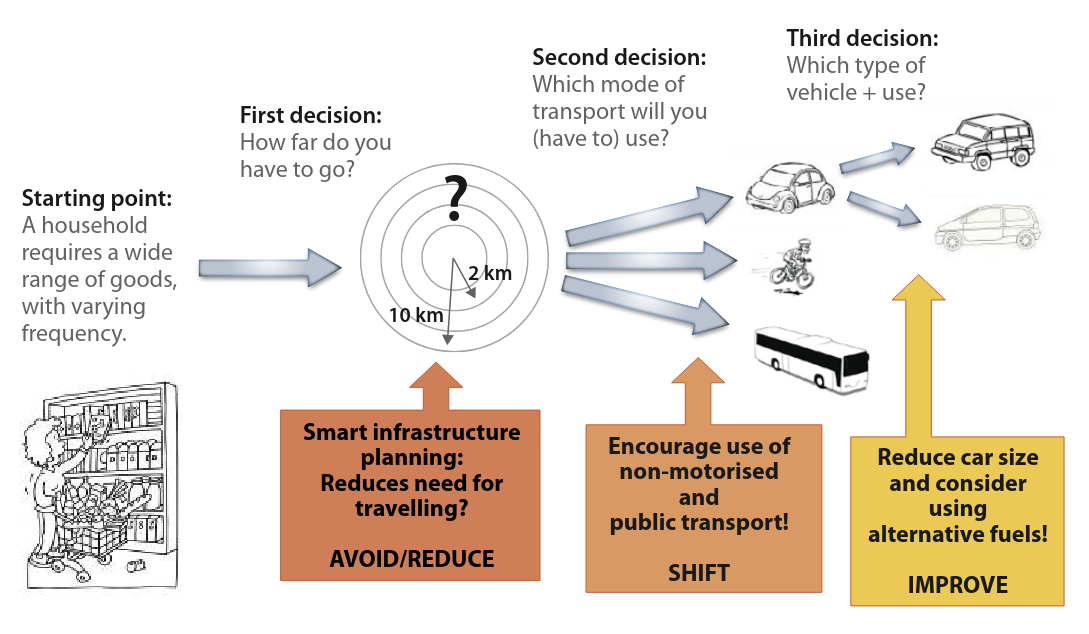
\includegraphics[width=0.94\linewidth]{images/avoidshiftimprove.png}
	\end{figure}

	\tiny\url{https://www.ledsgp.org/app/uploads/2016/01/SUTP_GIZ_FS_Avoid-Shift-Improve_EN.pdf}
	
\end{frame}



\begin{frame}
	
	\begin{figure}
		
		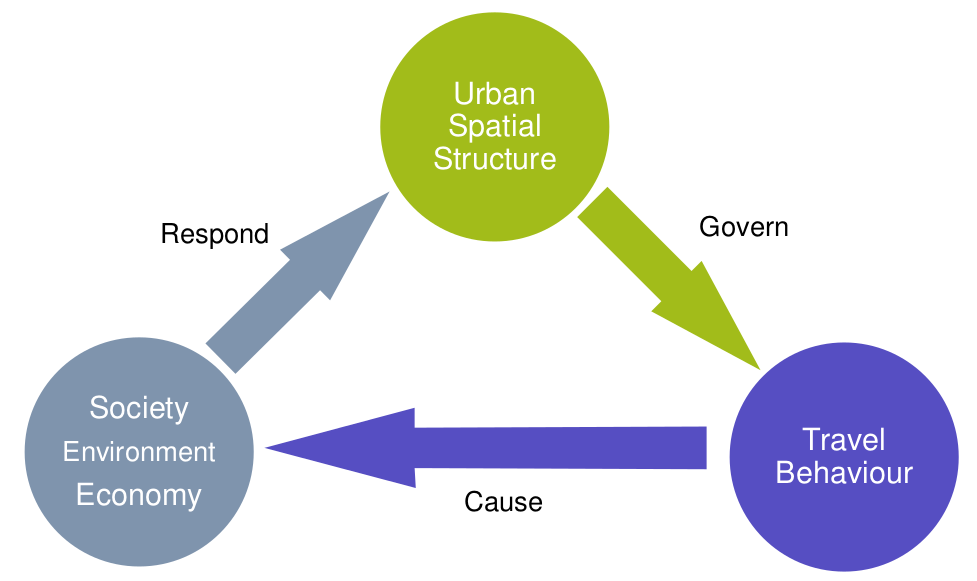
\includegraphics[width=0.94\linewidth]{images/big_links.png}
	\end{figure}
	
\end{frame}







\begin{frame}

	\begin{columns}
	
	
	
	\begin{column}{0.5\textwidth}
		
		\textbf{e.g. Milton, ON}
		
		\vspace{2mm}
		{Single-occupancy KM travelled per person per day}
		
		\begin{itemize}
			\item Milton = 29.4km
			\item GGH = 19.6km
		\end{itemize}
		
		\vspace{3mm}
		
	{Mode Share}
		
		\begin{figure}

			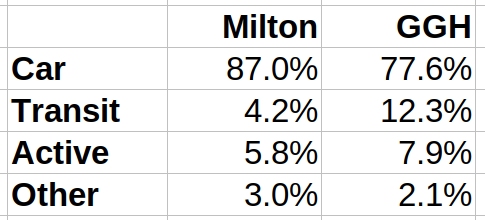
\includegraphics[width=1.02\linewidth]{images/milton-mode-share.png}
		\end{figure}
		
	\end{column}
	
	\begin{column}{0.5\textwidth}
		
	\begin{figure}

		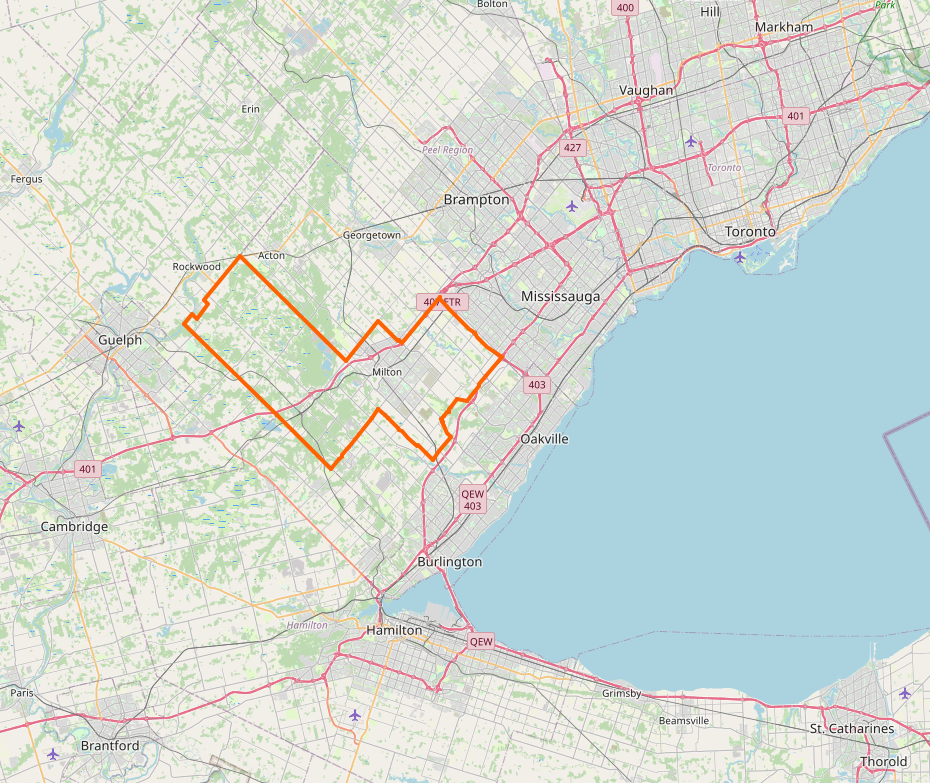
\includegraphics[width=0.64\linewidth]{images/milton.png}
	\end{figure}
	
		
		
	\end{column}
	
	\end{columns}

\end{frame}





\begin{frame}
	
	What about urban freight and deliveries?
	
	\begin{figure}
		
		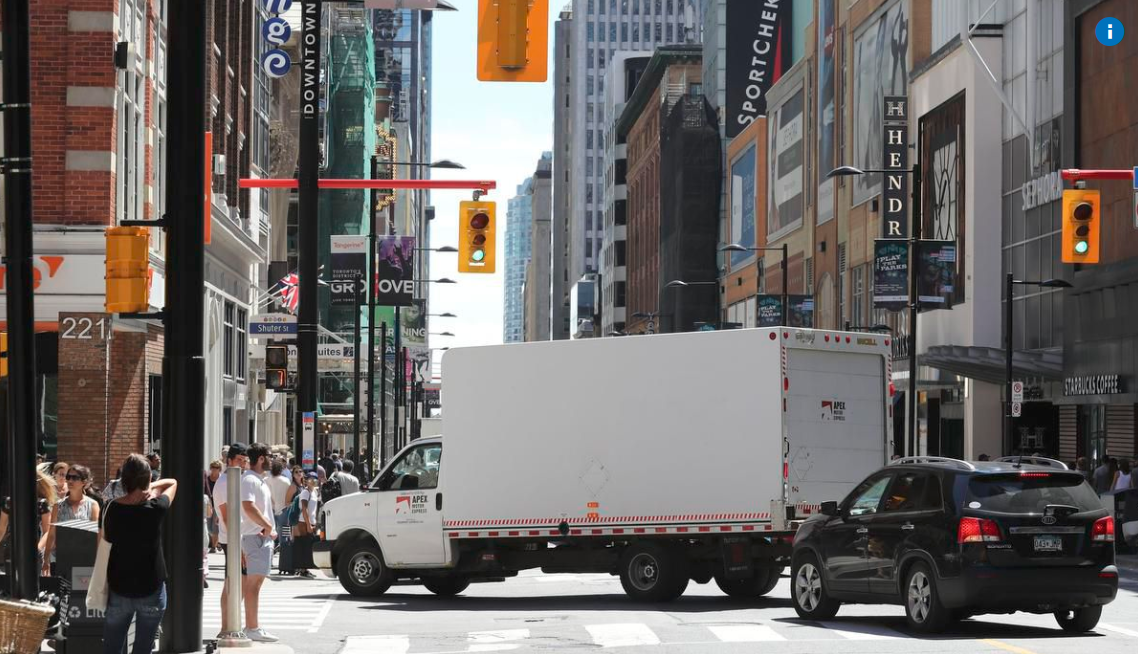
\includegraphics[width=0.87\linewidth]{images/delivery.png}
		
	\end{figure}

	\tiny \url{https://www.thestar.com/news/city_hall/2020/10/09/everyone-is-getting-everything-delivered-these-days-but-that-can-cause-chaos-on-city-streets-and-toronto-officials-are-trying-to-change-that.html?rf}
	
\end{frame}




\begin{frame}
	
	\textbf{Office Hours}
	
	\begin{itemize}
		
		\item Monday 3:30pm to 5:00pm (in-person SS5060 and Zoom)
		\item Friday 2:30pm to 3:30pm (only on Zoom)
	\end{itemize}
	
	
	\textbf{Next week}
	
	\begin{itemize}
		\item Health \& Equity
		\item How the costs and benefits of transportation are (in)equitably distributed
		\item Health impacts of	transportation (e.g. pollution, noise)
	\end{itemize}
	
\end{frame}



\end{document}